\documentclass[11pt,addpoints,answers]{exam}


%%%%%%%%%%%%%%%%%%%%%%%%%%%%%%%%%%%%%%%%%%%
% Commands for customizing the assignment %
%%%%%%%%%%%%%%%%%%%%%%%%%%%%%%%%%%%%%%%%%%%
\newcommand{\hwNum}{Homework 8}
\newcommand{\hwTopic}{Reinforcement Learning}
\newcommand{\hwName}{\hwNum: \hwTopic}
\newcommand{\outDate}{Sunday, November 16}
\newcommand{\dueDate}{Monday, November 24 at 11:59 PM}
\newcommand{\taNames}{Santiago, Akhil, Doris, Joyce, Markov, Neural}
\newcommand{\homeworktype}{\string written+prog}
\newcommand{\exitPollLink}{\string https://forms.gle/HfRddNmv4WjFRhXL7}
\newcommand{\usesPytorch}{\boolean true}

\newcommand{\summary}{
    \begin{notebox}
        \paragraph{Summary} In this assignment, you will use reinforcement learning to train an agent to play the classic Atari game Pong. As a warmup, the first section will lead you through an on-paper example of how value iteration and Q-learning work. Then, in Section \ref{sec:code}, you will implement the Advantage Actor Critic algorithm in pytorch to train an agent for the Pong enviroment.
    \end{notebox}
}


%% To HIDE SOLUTIONS (to post at the website for students), set this value to 0: \def\issoln{0}
\providecommand{\issoln}{1}
% \providecommand{\issoln}{0}

 %-----------------------------------------------------------------------------
% PACKAGES AND OTHER DOCUMENT CONFIGURATIONS
%-----------------------------------------------------------------------------

\usepackage[margin=1in]{geometry}
\usepackage{bbm}
\usepackage{amsmath, amsfonts}
\usepackage{enumerate}
\usepackage{graphicx}
\usepackage{titling}
\usepackage{url}
\usepackage{xfrac}
\usepackage{natbib}
\usepackage{amssymb}
\usepackage{amsthm}
\usepackage{paralist}
\usepackage{epstopdf}
\usepackage{tabularx}
\usepackage{longtable}
\usepackage{multirow}
\usepackage{multicol}
\usepackage[colorlinks=true,urlcolor=blue]{hyperref}
\usepackage{algorithm}
\usepackage{algorithmicx}
\usepackage[noend]{algpseudocode}
\usepackage{float}
\usepackage{enumerate}
\usepackage{array}
\usepackage{environ}
\usepackage{times}
\usepackage{textcomp}
\usepackage{caption}
\usepackage{parskip} % For NIPS style paragraphs.
\usepackage[compact]{titlesec} % Less whitespace around titles
\usepackage[inline]{enumitem} % For inline enumerate* and itemize*
\usepackage{datetime2}
\usepackage{comment}
% \usepackage{minted}
\usepackage{lastpage}
\usepackage{color}
\usepackage{xcolor}
\usepackage[final]{listings}
\usepackage{framed}
\usepackage{booktabs}
\usepackage{cprotect}
\usepackage{verbatim}
\usepackage{verbatimbox}
\usepackage{multicol}
\usepackage{hyperref}
\usepackage{subcaption}
\usepackage{mathtools} % For drcases
\usepackage{cancel}
\usepackage[many]{tcolorbox}
\usepackage{soul}
\usepackage[bottom]{footmisc}
\usepackage{bm}
\usepackage{wasysym}
\usepackage{pgfplots}
\usepackage{tikz}
\usetikzlibrary{shapes,decorations,arrows}
\usetikzlibrary{arrows.meta}
\usetikzlibrary{shapes.geometric}
\usetikzlibrary{positioning, arrows, automata, calc}
\usepackage{transparent}
\usepackage{tikz-cd}
\usepackage{setspace}


\newtcolorbox[]{your_solution}[1][]{
    % breakable,
    enhanced,
    nobeforeafter,
    colback=white,
    title=Your Answer,
    sidebyside align=top,
    box align=top,
    #1
}


%%%%%%%%%%%%%%%%%%%%%%%%%%%%%%%%%%%%%%%%%%%
% Rotated Column Headers                  %
%%%%%%%%%%%%%%%%%%%%%%%%%%%%%%%%%%%%%%%%%%%
\usepackage{adjustbox}
\usepackage{array}

%https://tex.stackexchange.com/questions/32683/rotated-column-titles-in-tabular

\newcolumntype{R}[2]{%
    >{\adjustbox{angle=#1,lap=\width-(#2)}\bgroup}%
    l%
    <{\egroup}%
}
\newcommand*\rot{\multicolumn{1}{R{45}{1em}}}% no optional argument here, please!


%%%%%%%%%%%%%%%%%%%%%%%%%%%%%%%%%%%%%%%%%%%
% Formatting for \CorrectChoice of "exam" %
%%%%%%%%%%%%%%%%%%%%%%%%%%%%%%%%%%%%%%%%%%%

\CorrectChoiceEmphasis{}
\checkedchar{\blackcircle}

\newenvironment{checkboxessquare}{
    \begingroup
    \checkboxchar{$\Box$} \checkedchar{$\blacksquare$} % change checkbox style locally
    \begin{checkboxes}
    }{
    \end{checkboxes}
    \endgroup
    }

%%%%%%%%%%%%%%%%%%%%%%%%%%%%%%%%%%%%%%%%%%%
% Better numbering                        %
%%%%%%%%%%%%%%%%%%%%%%%%%%%%%%%%%%%%%%%%%%%

% \numberwithin{equation}{section} % Number equations within sections (i.e. 1.1, 1.2, 2.1, 2.2 instead of 1, 2, 3, 4)
% \numberwithin{figure}{section} % Number figures within sections (i.e. 1.1, 1.2, 2.1, 2.2 instead of 1, 2, 3, 4)
% \numberwithin{table}{section} % Number tables within sections (i.e. 1.1, 1.2, 2.1, 2.2 instead of 1, 2, 3, 4)

%%%%%%%%%%%%%%%%%%%%%%%%%%%%%%%%%%%%%%%%%%
% Custom commands                        %
%%%%%%%%%%%%%%%%%%%%%%%%%%%%%%%%%%%%%%%%%%
\newcommand{\R}{\mathbb{R}}
\newcommand{\blackcircle}{\tikz\draw[black,fill=black] (0,0) circle (1ex);}
\renewcommand{\circle}{\tikz\draw[black] (0,0) circle (1ex);}


%%%%%%%%%%%%%%%%%%%%%%%%%%%%%%%%%%%%%%%%%%
% Custom commands for Math               %
%%%%%%%%%%%%%%%%%%%%%%%%%%%%%%%%%%%%%%%%%%
\newcommand{\vc}[1]{\boldsymbol{#1}}
\newcommand{\adj}[1]{\frac{\partial \ell}{\partial #1}}
\newcommand{\chain}[2]{\adj{#2} = \adj{#1}\frac{\partial #1}{\partial #2}}
\newcommand{\ntset}{test}
\newcommand{\zerov}{\mathbf{0}}
\DeclareMathOperator*{\argmin}{argmin}

% mathcal
\newcommand{\Ac}{\mathcal{A}}
\newcommand{\Bc}{\mathcal{B}}
\newcommand{\Cc}{\mathcal{C}}
\newcommand{\Dc}{\mathcal{D}}
\newcommand{\Ec}{\mathcal{E}}
\newcommand{\Fc}{\mathcal{F}}
\newcommand{\Gc}{\mathcal{G}}
\newcommand{\Hc}{\mathcal{H}}
\newcommand{\Ic}{\mathcal{I}}
\newcommand{\Jc}{\mathcal{J}}
\newcommand{\Kc}{\mathcal{K}}
\newcommand{\Lc}{\mathcal{L}}
\newcommand{\Mc}{\mathcal{M}}
\newcommand{\Nc}{\mathcal{N}}
\newcommand{\Oc}{\mathcal{O}}
\newcommand{\Pc}{\mathcal{P}}
\newcommand{\Qc}{\mathcal{Q}}
\newcommand{\Rc}{\mathcal{R}}
\newcommand{\Sc}{\mathcal{S}}
\newcommand{\Tc}{\mathcal{T}}
\newcommand{\Uc}{\mathcal{U}}
\newcommand{\Vc}{\mathcal{V}}
\newcommand{\Wc}{\mathcal{W}}
\newcommand{\Xc}{\mathcal{X}}
\newcommand{\Yc}{\mathcal{Y}}
\newcommand{\Zc}{\mathcal{Z}}

% mathbb
\newcommand{\Ab}{\mathbb{A}}
\newcommand{\Bb}{\mathbb{B}}
\newcommand{\Cb}{\mathbb{C}}
\newcommand{\Db}{\mathbb{D}}
\newcommand{\Eb}{\mathbb{E}}
\newcommand{\Fb}{\mathbb{F}}
\newcommand{\Gb}{\mathbb{G}}
\newcommand{\Hb}{\mathbb{H}}
\newcommand{\Ib}{\mathbb{I}}
\newcommand{\Jb}{\mathbb{J}}
\newcommand{\Kb}{\mathbb{K}}
\newcommand{\Lb}{\mathbb{L}}
\newcommand{\Mb}{\mathbb{M}}
\newcommand{\Nb}{\mathbb{N}}
\newcommand{\Ob}{\mathbb{O}}
\newcommand{\Pb}{\mathbb{P}}
\newcommand{\Qb}{\mathbb{Q}}
\newcommand{\Rb}{\mathbb{R}}
\newcommand{\Sb}{\mathbb{S}}
\newcommand{\Tb}{\mathbb{T}}
\newcommand{\Ub}{\mathbb{U}}
\newcommand{\Vb}{\mathbb{V}}
\newcommand{\Wb}{\mathbb{W}}
\newcommand{\Xb}{\mathbb{X}}
\newcommand{\Yb}{\mathbb{Y}}
\newcommand{\Zb}{\mathbb{Z}}

% mathbf lowercase
\newcommand{\av}{\mathbf{a}}
\newcommand{\bv}{\mathbf{b}}
\newcommand{\cv}{\mathbf{c}}
\newcommand{\dv}{\mathbf{d}}
\newcommand{\ev}{\mathbf{e}}
\newcommand{\fv}{\mathbf{f}}
\newcommand{\gv}{\mathbf{g}}
\newcommand{\hv}{\mathbf{h}}
\newcommand{\iv}{\mathbf{i}}
\newcommand{\jv}{\mathbf{j}}
\newcommand{\kv}{\mathbf{k}}
\newcommand{\lv}{\mathbf{l}}
\newcommand{\mv}{\mathbf{m}}
\newcommand{\nv}{\mathbf{n}}
\newcommand{\ov}{\mathbf{o}}
\newcommand{\pv}{\mathbf{p}}
\newcommand{\qv}{\mathbf{q}}
\newcommand{\rv}{\mathbf{r}}
\newcommand{\sv}{\mathbf{s}}
\newcommand{\tv}{\mathbf{t}}
\newcommand{\uv}{\mathbf{u}}
\newcommand{\vv}{\mathbf{v}}
\newcommand{\wv}{\mathbf{w}}
\newcommand{\xv}{\mathbf{x}}
\newcommand{\yv}{\mathbf{y}}
\newcommand{\zv}{\mathbf{z}}

% mathbf uppercase
\newcommand{\Av}{\mathbf{A}}
\newcommand{\Bv}{\mathbf{B}}
\newcommand{\Cv}{\mathbf{C}}
\newcommand{\Dv}{\mathbf{D}}
\newcommand{\Ev}{\mathbf{E}}
\newcommand{\Fv}{\mathbf{F}}
\newcommand{\Gv}{\mathbf{G}}
\newcommand{\Hv}{\mathbf{H}}
\newcommand{\Iv}{\mathbf{I}}
\newcommand{\Jv}{\mathbf{J}}
\newcommand{\Kv}{\mathbf{K}}
\newcommand{\Lv}{\mathbf{L}}
\newcommand{\Mv}{\mathbf{M}}
\newcommand{\Nv}{\mathbf{N}}
\newcommand{\Ov}{\mathbf{O}}
\newcommand{\Pv}{\mathbf{P}}
\newcommand{\Qv}{\mathbf{Q}}
\newcommand{\Rv}{\mathbf{R}}
\newcommand{\Sv}{\mathbf{S}}
\newcommand{\Tv}{\mathbf{T}}
\newcommand{\Uv}{\mathbf{U}}
\newcommand{\Vv}{\mathbf{V}}
\newcommand{\Wv}{\mathbf{W}}
\newcommand{\Xv}{\mathbf{X}}
\newcommand{\Yv}{\mathbf{Y}}
\newcommand{\Zv}{\mathbf{Z}}

% bold greek lowercase
\newcommand{\alphav     }{\boldsymbol \alpha     }
\newcommand{\betav      }{\boldsymbol \beta      }
\newcommand{\gammav     }{\boldsymbol \gamma     }
\newcommand{\deltav     }{\boldsymbol \delta     }
\newcommand{\epsilonv   }{\boldsymbol \epsilon   }
\newcommand{\varepsilonv}{\boldsymbol \varepsilon}
\newcommand{\zetav      }{\boldsymbol \zeta      }
\newcommand{\etav       }{\boldsymbol \eta       }
\newcommand{\thetav     }{\boldsymbol \theta     }
\newcommand{\varthetav  }{\boldsymbol \vartheta  }
\newcommand{\iotav      }{\boldsymbol \iota      }
\newcommand{\kappav     }{\boldsymbol \kappa     }
\newcommand{\varkappav  }{\boldsymbol \varkappa  }
\newcommand{\lambdav    }{\boldsymbol \lambda    }
\newcommand{\muv        }{\boldsymbol \mu        }
\newcommand{\nuv        }{\boldsymbol \nu        }
\newcommand{\xiv        }{\boldsymbol \xi        }
\newcommand{\omicronv   }{\boldsymbol \omicron   }
\newcommand{\piv        }{\boldsymbol \pi        }
\newcommand{\varpiv     }{\boldsymbol \varpi     }
\newcommand{\rhov       }{\boldsymbol \rho       }
\newcommand{\varrhov    }{\boldsymbol \varrho    }
\newcommand{\sigmav     }{\boldsymbol \sigma     }
\newcommand{\varsigmav  }{\boldsymbol \varsigma  }
\newcommand{\tauv       }{\boldsymbol \tau       }
\newcommand{\upsilonv   }{\boldsymbol \upsilon   }
\newcommand{\phiv       }{\boldsymbol \phi       }
\newcommand{\varphiv    }{\boldsymbol \varphi    }
\newcommand{\chiv       }{\boldsymbol \chi       }
\newcommand{\psiv       }{\boldsymbol \psi       }
\newcommand{\omegav     }{\boldsymbol \omega     }

% bold greek uppercase
\newcommand{\Gammav     }{\boldsymbol \Gamma     }
\newcommand{\Deltav     }{\boldsymbol \Delta     }
\newcommand{\Thetav     }{\boldsymbol \Theta     }
\newcommand{\Lambdav    }{\boldsymbol \Lambda    }
\newcommand{\Xiv        }{\boldsymbol \Xi        }
\newcommand{\Piv        }{\boldsymbol \Pi        }
\newcommand{\Sigmav     }{\boldsymbol \Sigma     }
\newcommand{\Upsilonv   }{\boldsymbol \Upsilon   }
\newcommand{\Phiv       }{\boldsymbol \Phi       }
\newcommand{\Psiv       }{\boldsymbol \Psi       }
\newcommand{\Omegav     }{\boldsymbol \Omega     }

%%%%%%%%%%%%%%%%%%%%%%%%%%%%%%%%%%%%%%%%%%%
% Code highlighting with listings         %
%%%%%%%%%%%%%%%%%%%%%%%%%%%%%%%%%%%%%%%%%%%

\definecolor{bluekeywords}{rgb}{0.13,0.13,1}
\definecolor{greencomments}{rgb}{0,0.5,0}
\definecolor{redstrings}{rgb}{0.9,0,0}
\definecolor{light-gray}{gray}{0.95}

\newcommand{\MYhref}[3][blue]{\href{#2}{\color{#1}{#3}}}%

\definecolor{dkgreen}{rgb}{0,0.6,0}
\definecolor{gray}{rgb}{0.5,0.5,0.5}
\definecolor{mauve}{rgb}{0.58,0,0.82}

\lstdefinelanguage{Shell}{
  keywords={tar, cd, make},
  %keywordstyle=\color{bluekeywords}\bfseries,
  alsoletter={+},
  ndkeywords={python, py, javac, java, gcc, c, g++, cpp, .txt, octave, m, .tar},
  %ndkeywordstyle=\color{bluekeywords}\bfseries,
  identifierstyle=\color{black},
  sensitive=false,
  comment=[l]{//},
  morecomment=[s]{/*}{*/},
  commentstyle=\color{purple}\ttfamily,
  %stringstyle=\color{red}\ttfamily,
  morestring=[b]',
  morestring=[b]",
  backgroundcolor = \color{light-gray}
}

\lstset{columns=fixed, basicstyle=\ttfamily,
    backgroundcolor=\color{light-gray},xleftmargin=0.5cm,frame=tlbr,framesep=4pt,framerule=0pt}

\newcommand{\emptysquare}{{\LARGE $\square$}\ \ }
\newcommand{\filledsquare}{{\LARGE $\boxtimes$}\ \ }
\def \ifempty#1{\def\temp{#1} \ifx\temp\empty }

\def \squaresolutionspace#1{ \ifempty{#1} \emptysquare \else #1\hspace{0.75pt}\fi}

\newcommand{\emptycircle}{{\LARGE $\fullmoon$}\ \ }
\newcommand{\filledcircle}{{\LARGE $\newmoon$}\ \ }
\def \circlesolutionspace#1{ \ifempty{#1} \emptycircle \else #1\hspace{0.75pt}\fi}

%%%%%%%%%%%%%%%%%%%%%%%%%%%%%%%%%%%%%%%%%%%
% Custom box for highlights               %
%%%%%%%%%%%%%%%%%%%%%%%%%%%%%%%%%%%%%%%%%%%

% Define box and box title style
\tikzstyle{mybox} = [fill=blue!10, very thick,
    rectangle, rounded corners, inner sep=1em, inner ysep=1em]

% \newcommand{\notebox}[1]{
% \begin{tikzpicture}
% \node [mybox] (box){%
%     \begin{minipage}{\textwidth}
%     #1
%     \end{minipage}
% };
% \end{tikzpicture}%
% }

\NewEnviron{notebox}{

\begin{tikzpicture}
\node [mybox] (box){
    \begin{minipage}{\textwidth}
        \BODY
    \end{minipage}
};
\end{tikzpicture}
}

%%%%%%%%%%%%%%%%%%%%%%%%%%%%%%%%%%%%%%%%%%%
% Commands showing / hiding solutions     %
%%%%%%%%%%%%%%%%%%%%%%%%%%%%%%%%%%%%%%%%%%%

%%%%%%%%%%%%%%%%%%%%%%%%%%%%%%%%%%%%%%%%%%%
% Commands showing / hiding solutions     %
%%%%%%%%%%%%%%%%%%%%%%%%%%%%%%%%%%%%%%%%%%%
\newcommand{\solutionspace}[4]{\fbox{\begin{minipage}[t][#1][t]{#2} \textbf{#3} \solution{}{#4} \end{minipage}}}

%% To HIDE SOLUTIONS (to post at the website for students), set this value to 0: \def\issoln{0}
% \def\issoln{0} % Uncomment to remove solutions
% \def\issoln{1} % Uncomment to show solutions

% Some commands to allow solutions to be embedded in the assignment file.
\ifcsname issoln\endcsname \else \def\issoln{1} \fi

% Default to an empty solutions environ.
\NewEnviron{soln}{}{}
\if\issoln 1

% Otherwise, include solutions as below.
 \RenewEnviron{soln}{
    \leavevmode\color{red}\ignorespaces   %textbf{Solution} \BODY
    \BODY
 }{}
\fi

%%%%%%%%%%%%%%%%

%% qauthor environment:
% Default to an empty qauthor environ.
\NewEnviron{qauthor}{}{}

%% To HIDE TAGS set this value to 0:
\def\showtags{0}  % Uncomment to remove tags
% \def\showtags{1} % Uncomment to show tags


\ifcsname showtags\endcsname \else \def\showtags{1} \fi

% Default to an empty tags environ.
\NewEnviron{tags}{}{}
\if\showtags 1

% Otherwise, include solutions as below.
\RenewEnviron{tags}{
    \fbox{
    \leavevmode\color{blue}\ignorespaces
    \textbf{TAGS:} \texttt{\url{\BODY}}
    }
    \vspace{-.5em}
}{}
\fi

% Default to an empty learning objective environment
\NewEnviron{qlearningobjective}{}
%%%%%%%%%%%%%%%%%%%%%%%%%%%%%%%%%%%%%%%%%%%%%%%%%
% Useful commands for typesetting the questions %
%%%%%%%%%%%%%%%%%%%%%%%%%%%%%%%%%%%%%%%%%%%%%%%%%

\newcommand \expect {\mathbb{E}}
\newcommand \mle [1]{{\hat #1}^{\rm MLE}}
\newcommand \map [1]{{\hat #1}^{\rm MAP}}
\newcommand \argmax {\operatorname*{argmax}}
% \newcommand \argmin {\operatorname*{argmin}}
\newcommand \code [1]{{\tt #1}}
\newcommand \datacount [1]{\#\{#1\}}
\newcommand \ind [1]{\mathbb{I}\{#1\}}

%%%%%%%%%%%%%%%%%%%%%%%%%%
% Document configuration %
%%%%%%%%%%%%%%%%%%%%%%%%%%

% Don't display a date in the title and remove the white space
\predate{}
\postdate{}
\date{}

% Don't display an author and remove the white space
%\preauthor{}
%\postauthor{}

% Solo and group questions
\newcommand{\solo}{\textbf{[SOLO]} }
\newcommand{\group}{\textbf{[GROUP]} }

% Question type commands
\newcommand{\sall}{\textbf{Select all that apply: }}
\newcommand{\sone}{\textbf{Select one: }}
\newcommand{\tf}{\textbf{True or False: }}

% AdaBoost commands
\newcommand{\trainerr}[1]{\hat{\epsilon}_S \left(#1\right)}
\newcommand{\generr}[1]{\epsilon \left(#1\right)}
\newcommand{\D}{\mathcal{D}}
\newcommand{\margin}{\text{margin}}
\newcommand{\sign}{\text{sign}}
\newcommand{\PrS}{\hat{\Pr_{(x_i, y_i) \sim S}}}
\newcommand{\PrSinline}{\hat{\Pr}_{(x_i, y_i) \sim S}}  % inline PrS

% Abhi messing around with examdoc
\qformat{\textbf{{\Large \thequestion \; \; \thequestiontitle \ (\totalpoints \ points)}} \hfill}
\renewcommand{\thequestion}{\arabic{question}}
\renewcommand{\questionlabel}{\thequestion.}

\renewcommand{\thepartno}{\arabic{partno}}
\renewcommand{\partlabel}{\thepartno.}
\renewcommand{\partshook}{\setlength{\leftmargin}{0pt}}

\renewcommand{\thesubpart}{\alph{subpart}}
\renewcommand{\subpartlabel}{(\thesubpart)}

\renewcommand{\thesubsubpart}{\roman{subsubpart}}
\renewcommand{\subsubpartlabel}{\thesubsubpart.}

% copied from stack overflow, as all good things are
\newcommand\invisiblesection[1]{%
  \refstepcounter{section}%
  \addcontentsline{toc}{section}{\protect\numberline{\thesection}#1}%
  \sectionmark{#1}}

% quite possibly the worst workaround i have made for this class
\newcommand{\sectionquestion}[1]{
\titledquestion{#1}
\invisiblesection{#1}
~\vspace{-1em}
}

% also copied from stack overflow
% https://tex.stackexchange.com/questions/153846/indent-every-subsubsection-element
% and edited following
% https://latexref.xyz/bs-at-startsection.html
% PLEASE DELETE THIS FOR OTHER HOMEWORK
% \ifnum\pdfstrcmp{\taNames}{Sana, Chu, Hayden, Tori, Prasoon}=0
% \makeatletter
% \newcommand\subsectionquestion{%
%   \@startsection{subsection}{2}
%   {-2pc}% <------- The opposite of what we set for subs
%   {-3.25ex\@plus -1ex \@minus -.2ex}%
%   {1.5ex \@plus .2ex}%
%   {\normalfont\large\bfseries}}
% \makeatother
% \fi

%%%%%%%%%%%%%%%%%%%%%%%%%%%%%%%%%%%%%%%%%%%
% New Environment for Pseudocode          %
%%%%%%%%%%%%%%%%%%%%%%%%%%%%%%%%%%%%%%%%%%%

% Python style for highlighting
\DeclareFixedFont{\ttb}{T1}{txtt}{bx}{n}{12} % for bold
\DeclareFixedFont{\ttm}{T1}{txtt}{m}{n}{12}  % for normal

\definecolor{deepblue}{rgb}{0,0,0.5}
\definecolor{deepred}{rgb}{0.6,0,0}
\definecolor{deepgreen}{rgb}{0,0.5,0}

\newcommand\pythonstyle{\lstset{
language=Python,
basicstyle=\ttm,
morekeywords={self},              % Add keywords here
keywordstyle=\ttb\color{deepblue},
emph={MyClass,__init__},          % Custom highlighting
emphstyle=\ttb\color{deepred},    % Custom highlighting style
stringstyle=\color{deepgreen},
frame=tb,                         % Any extra options here
showstringspaces=false
}}


% Python environment
\lstnewenvironment{your_code_solution}[1][]
{
\pythonstyle
\lstset{#1}
}
{}
\newtcolorbox[]{your_code_solution_outer}[1][]{
    % breakable,
    enhanced,
    nobeforeafter,
    colback=white,
    title=Your Answer,
    sidebyside align=top,
    box align=top,
    #1
}
%%%%%%%%%%%%%%%%%%%%%%%%%%%%%%%%%%%%%%%%%%%
% Commands for customizing the assignment %
%%%%%%%%%%%%%%%%%%%%%%%%%%%%%%%%%%%%%%%%%%%
\newcommand{\courseNum}{10-301 / 10-601}
\newcommand{\courseName}{Introduction to Machine Learning}
\newcommand{\courseSem}{Fall 2025}
\newcommand{\courseUrl}{\url{http://www.cs.cmu.edu/~mgormley/courses/10601/}}

%\pagestyle{fancyplain}
\lhead{\hwName}
\rhead{\courseNum}
\cfoot{\thepage{} of \numpages{}}

\title{\textsc{\hwNum}: \textsc{\hwTopic} 
\thanks{Compiled on \today{} at \DTMcurrenttime{}}\\
\vspace{1em}
} % Title

\author{\textsc{\large \courseNum{} \courseName{} (\courseSem)}\\
\courseUrl
\vspace{1em}\\
  OUT: \outDate \\
  DUE: \dueDate \\
  TAs: \taNames\\
}

\date{}
\begin{document}
    \maketitle
    \summary{}
    
\section*{START HERE: Instructions}
\begin{itemize}
\newcommand \maxsubs {10 }

\item \textbf{Collaboration Policy}: Please read the collaboration policy here: \url{http://mlcourse.org/index.html#7-collaboration-and-academic-integrity-policies}

\item\textbf{Late Submission Policy:} See the late submission policy here: \url{http://mlcourse.org/index.html#6-general-policies}

\item\textbf{Submitting your work:} You will use Gradescope to submit
  answers to all questions\ifthenelse{\equal{\homeworktype}{\string written}}{}{ and code. Please
  follow instructions at the end of this PDF to correctly submit all your code to Gradescope}.

\begin{itemize}
    \item \textbf{Written:} For written problems such as short answer, multiple choice, derivations, proofs, or plots, please use the provided template. Submissions can be handwritten onto the template, but should be labeled and clearly legible. If your writing is not legible, you will not be awarded marks. Alternatively, submissions can be written in \LaTeX{}. Each derivation/proof should be completed in the boxes provided. You are responsible for ensuring that your submission contains exactly the same number of pages and the same alignment as our PDF template. If you do not follow the template, your assignment may not be graded correctly by our AI assisted grader and there will be a \textbf{\textcolor{red}{2\% penalty}} (e.g., if the homework is out of 100 points, 2 points will be deducted from your final score).

    % This policy is NOT in effect when we have the Background Test.
    \ifthenelse{\equal{\hwNum}{Homework 1}}{ {\color{red} For this assignment only, if you answer at least 90\% of the written questions correctly, you get full marks on the written portion of this assignment. For this assignment only, \textbf{we will offer two rounds of grading}. The first round of grading will happen immediately following the due date specified above. We will then release your grades to you and if you got less than 90\% on the written questions, you will be allowed to submit once again by a second due date. The exact due date for the second round will be announced after we release the first round grades. } }{}

    \ifthenelse{\equal{\homeworktype}{\string written}}{}{
    \item \textbf{Programming:} You will submit your code for programming questions on the homework to \href{https://gradescope.com}{Gradescope}. After uploading your code, our grading scripts will autograde your assignment by running your program on a virtual machine (VM). 
    %
    You are only permitted to use \ifthenelse{\equal{\usesPytorch}{\boolean true}}{Pytorch modules (see writeup for fully authorized list), }{}\href{https://docs.python.org/3/library/}{the Python Standard Library modules} and \texttt{numpy}.
    
    % You are only permitted to use \href{https://docs.python.org/3/library/}{the Python Standard Library modules}, \texttt{numpy} and the modules already imported in the starter notebook. You are not permitted to import any other modules.
    %
    % You will not have to change the default version of your programming environment and the versions of the permitted libraries on Google Colab. You have \maxsubs free Gradescope programming submissions, after which you will begin to lose points from your total programming score. We recommend debugging your implementation on Google Colab and making sure your code is running correctly first before submitting your code to Gradescope.}
    %
    Ensure that the version number of your programming language environment (i.e. Python 3.12.*) and versions of permitted libraries (i.e. \texttt{numpy} 2.2.4) match those used on Gradescope. You have \maxsubs free Gradescope programming submissions, after which you will begin to lose points from your total programming score. We recommend debugging your implementation on your local machine (or the Linux servers) and making sure your code is running correctly first before submitting your code to Gradescope.}
    \ifthenelse{\equal{\hwNum Homework 1} {{\color{red} The submission limit is true for future assignments, but this one allows \textbf{unlimited submissions.}}}} {}
   
  \end{itemize}
  
\ifthenelse{\equal{\homeworktype}{\string written}}{}{\item\textbf{Materials:} The data and reference output that you will need in order to complete this assignment is posted along with the writeup and template on the course website.}

\end{itemize}

\pagebreak

    \clearpage
    
\section*{Instructions for Specific Problem Types}

For ``Select One" questions, please fill in the appropriate bubble completely:

\begin{quote}
\textbf{Select One:} Who taught this course?
    \begin{checkboxes}
     \CorrectChoice Matt Gormley
     \choice Henry Chai
     \choice Noam Chomsky
    \end{checkboxes}
\end{quote}

If you need to change your answer, you may cross out the previous answer and bubble in the new answer:

\begin{quote}
\textbf{Select One:} Who taught this course?
    {
    \begin{checkboxes}
     \CorrectChoice Matt Gormley
     \choice Henry Chai \checkboxchar{\xcancel{\blackcircle}{}}
     \choice Noam Chomsky
    \end{checkboxes}
    }
\end{quote}

For ``Select all that apply" questions, please fill in all appropriate squares completely:

\begin{quote}
\textbf{Select all that apply:} Which are instructors for this course?
    {%
    \checkboxchar{$\Box$} \checkedchar{$\blacksquare$} % change checkbox style locally
    \begin{checkboxes}
    \CorrectChoice Matt Gormley  
    \CorrectChoice Geoff Gordon
    \choice Henry Chai
    \choice I don't know
    \end{checkboxes}
    }
\end{quote}

Again, if you need to change your answer, you may cross out the previous answer(s) and bubble in the new answer(s):

\begin{quote}
\textbf{Select all that apply:} Which are the instructors for this course?
    {%
    \checkboxchar{\xcancel{$\blacksquare$}} \checkedchar{$\blacksquare$} % change checkbox style locally
    \begin{checkboxes}
    \CorrectChoice Matt Gormley 
    \CorrectChoice Geoff Gordon
    \choice Henry Chai
    \choice I don't know
    \end{checkboxes}
    }
\end{quote}

For questions where you must fill in a blank, please make sure your final answer is fully included in the given space. You may cross out answers or parts of answers, but the final answer must still be within the given space.

\begin{quote}
\textbf{Fill in the blank:} What is the course number?

\begin{tcolorbox}[fit,height=1cm, width=4cm, blank, borderline={1pt}{-2pt},nobeforeafter]
    \begin{center}\huge10-601\end{center}
    \end{tcolorbox}\hspace{2cm}
    \begin{tcolorbox}[fit,height=1cm, width=4cm, blank, borderline={1pt}{-2pt},nobeforeafter]
    \begin{center}\huge10-\xcancel{6}301\end{center}
    \end{tcolorbox}
\end{quote}
    \clearpage
    
    {\LARGE \bf Written Questions (\numpoints \ points)}
    
    \begin{questions}
\sectionquestion{\LaTeX{} Point and Template Alignment}
\begin{parts}
    \part[1] \sone Did you use \LaTeX{} for the entire written portion of this homework?
    
    \begin{checkboxes}
        % YOUR ANSWER
        % Change \choice to \CorrectChoice for the appropriate selection/selections 
        \choice Yes 
        \choice No
    \end{checkboxes}

    \part[0] \sone I have ensured that my final submission is aligned with the original template given to me in the handout file and that I haven't deleted or resized any items or made any other modifications which will result in a misaligned template. I understand that incorrectly responding yes to this question will result in a penalty equivalent to 2\% of the points on this assignment.\\
    \textbf{Note:} Failing to answer this question will not exempt you from the 2\% misalignment penalty.
    
    \begin{checkboxes}
        % YOUR ANSWER
        % Change \choice to \CorrectChoice for the appropriate selection/selections 
        \choice Yes 
    \end{checkboxes}

    \part[0] \sone Did you fill out the \href{\exitPollLink}{Exit Poll} for the previous HW? Completing the exit poll will count towards your participation grade. 
    \begin{checkboxes}
        % YOUR ANSWER
        % Change \choice to \CorrectChoice for the appropriate selection/selections 
        \choice Yes 
    \end{checkboxes}
    
    \clearpage
\end{parts}
    \newpage
\sectionquestion{Value Iteration}

While attending an ML conference, you meet scientists at NASA who ask you to develop a reinforcement learning agent capable of carrying out a space-flight from Earth to the Sun.
You model this problem as a Markov decision process (MDP). The figure below depicts the state space. 

% \begin{center}
% \begin{tikzpicture}
% \draw[step=2cm] (0,0) grid (8, 6);

% \node at (4.5, 0.25) {Earth};
% \node at (6.5, 4.25) {Sun};
% \node at (0.5, 2.25) {Metis};

% \foreach \x/\y in {
%     2/1, 0/2, 0/0} ]
%     \draw[fill=white!50!gray] 
%     (2*\x,2*\y) rectangle (2*\x + 2, 2*\y + 2);


% \foreach \x/\y/\m in {
%     0/2/I, 1/2/J, 2/2/K, 3/2/L,
%     0/1/E, 1/1/F, 2/1/G, 3/1/H,
%     0/0/A, 1/0/B, 2/0/C, 3/0/D}
%     \node at (2*\x + 1.5,2*\y + 1.5) {$S_\m$};

% \node[state, draw=none] (n1) at (5, 4.7) {};
% \node[state, draw=none] (n2) at (7, 4.7) {};
% \node[state, draw=none] (n3) at (7, 3) {};
% \node[state, draw=none] (n4) at (1, 2.5) {};
% \node[state, draw=none] (n5) at (3, 2.5) {};

% \draw [->] (n1) to node[pos=0.5, above] {+50} (n2);
% \draw [->] (n3) to node[pos=0.4, left] {+25} (n2);
% \draw [->] (n5) to node[pos=0.5, below] {-50} (n4);

% \end{tikzpicture}
% \end{center}


\begin{center}
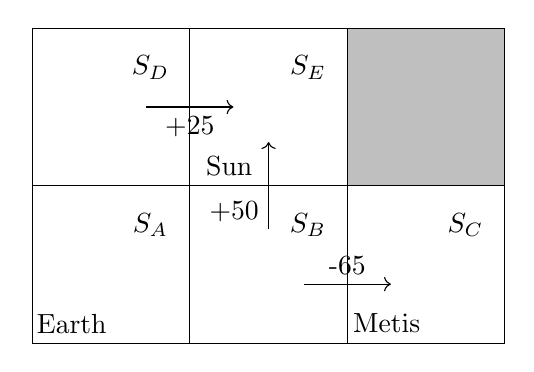
\begin{tikzpicture}
\draw[step=2cm] (0,0) grid (6, 4);



\node at (0.5, 0.25) {Earth};
\node at (2.5, 2.25) {Sun};
\node at (4.5, 0.25) {Metis};

\draw[fill=white!50!gray] (4,2) rectangle (6, 4);

\foreach \x/\y/\m in {
    0/1/D, 1/1/E,
    0/0/A, 1/0/B, 2/0/C}
    \node at (2*\x + 1.5,2*\y + 1.5) {$S_\m$};

\node[state, draw=none] (n0) at (3, 0.75) {};
\node[state, draw=none] (n1) at (5, 0.75) {};
\node[state, draw=none] (n2) at (3, 3) {};
\node[state, draw=none] (n3) at (3, 1) {};
\node[state, draw=none] (n4) at (1, 3) {};
\node[state, draw=none] (n5) at (3, 3) {};

\draw [->] (n0) to node[pos=0.5, above] {-65} (n1);
\draw [->] (n3) to node[pos=0.2, left] {+50} (n2);
\draw [->] (n4) to node[pos=0.5, below] {+25} (n5);

\end{tikzpicture}
\end{center}


Here are the details:

\begin{enumerate}
    \item Each grid cell is a state $S_A, S_B,..., S_E$ corresponding to a position in the solar system. The start state is $S_A$ (Earth). The terminal states include both the $S_E$ (Sun) and $S_C$ (Metis).
    \item The action space includes movement \texttt{up}/\texttt{down}/\texttt{left}/\texttt{right}. Transitions are \textbf{non-deterministic}. With probability $80\%$ the agent transitions to the intended state. With probability $10\%$ the agent slips left \emph{of the intended direction}. With probability $10\%$ the agent slips right \emph{of the intended direction}. In other words, we can think of \emph{the intended direction} as the direction \emph{the agent faces}, so the notions of \emph{left} and \emph{right} are based on the direction the agent faces. For example, if the agent is in state $S_B$ and takes action \texttt{left},  it moves to state $S_A$ with 80\% probability, it moves to state $S_B$ (left of the intended direction is down off the board, so the agent remains where it was) with 10\% probability, and it moves to state $S_E$ (right of the intended direction)  with 10\% probability.
    \item It is not possible to move to the blocked state (shaded grey) since it contains another planet. If the agent's action moves them off the board or to the blocked state, it remains in the same state.
    \item Non-zero rewards are depicted with arrows. Flying into the Sun from below gives positive reward $R(S_B, \texttt{a}, S_E) = +50$ $\forall \texttt{a} \in$ $\{\texttt{up},\texttt{down},\texttt{left},\texttt{right}\}$, since it is more fuel-efficient than flying into the sun from the left (the agent can use the gravitational field of the planet in the blocked state and Metis). However, approaching the Sun from below has risks, as flying too close to Metis is inadvisable and gives negative reward $R(S_B, \texttt{a}, S_C) = -65$ $\forall \texttt{a} \in$ $\{\texttt{up},\texttt{down},\texttt{left},\texttt{right}\}$. Note that flying into the Sun from the left still achieves the goal and gives positive reward $R(S_D, \texttt{a}, S_E) = +25$ $\forall \texttt{a} \in$ $\{\texttt{up},\texttt{down},\texttt{left},\texttt{right}\}$. All other rewards are zero.
\end{enumerate}

    
Below, let $V^*(s)$ denote the value function for state $s$ using the optimal policy $\pi^*(s)$.

\vspace{1em}
% \clearpage

\subsection{Synchronous Value Iteration}

\begin{parts}

    \part[3] Report the value of each state (including terminal states) after a single round of \textbf{synchronous} value iteration in the table below. Initialize the value table $V^0(s) = 0$, $\forall s \in \{S_A \hdots S_E\}$ and assume $\gamma=0.9$. Visit each state in \textit{reverse alphabetical order} (does this matter for synchronous value iteration?). Ignore the blocked states. Round your \textit{answers only} to the first decimal place. \textbf{Do not round intermediate values when calculating your answers.}
    
    
    \begin{center}
    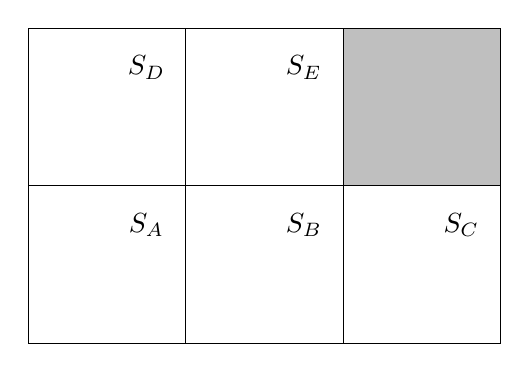
\begin{tikzpicture}
    \draw[step=2cm] (0,0) grid (6, 4);
    
    \draw[fill=white!50!gray] (4,2) rectangle (6, 4);
    
    \foreach \x/\y/\m in {
        0/1/D, 1/1/E, 
        0/0/A, 1/0/B, 2/0/C}
        \node at (2*\x + 1.5,2*\y + 1.5) {$S_\m$};

    % WRITE YOUR SOLUTION HERE
    % Be careful NOT TO DELETE THE COMMA!
    % There MUST be a comma at the end of every line
    \foreach \x/\y/\m in {
        0/0/{}, % REPLACE THE {} WITH THE VALUE FOR STATE A HERE 
        1/0/{}, % REPLACE THE {} WITH THE VALUE FOR STATE B HERE 
        2/0/{}, % REPLACE THE {} WITH THE VALUE FOR STATE C HERE 
        0/1/{}, % REPLACE THE {} WITH THE VALUE FOR STATE D HERE 
        1/1/{} % REPLACE THE {} WITH THE VALUE FOR STATE E HERE
        }  
        \node at (2*\x + 1,2*\y + 1) {$\m$};
    
    \end{tikzpicture}
    \end{center}


    % \begin{center}
    % \begin{tikzpicture}
    % \draw[step=2cm] (0,0) grid (8, 6);
    
    % \foreach \x/\y in {
    %     2/1, 0/2, 0/0}
    %     \draw[fill=white!50!gray] 
    %     (2*\x,2*\y) rectangle (2*\x + 2, 2*\y + 2);
    
    
    % \foreach \x/\y/\m in {
    %     0/2/I, 1/2/J, 2/2/K, 3/2/L,
    %     0/1/E, 1/1/F, 2/1/G, 3/1/H,
    %     0/0/A, 1/0/B, 2/0/C, 3/0/D}
    %     \node at (2*\x + 1.5,2*\y + 1.5) {$S_\m$};
        
    % % WRITE YOUR SOLUTION HERE
    % % Be careful NOT TO DELETE THE COMMA!
    % % There MUST be a comma at the end of every line
    % \foreach \x/\y/\m in {
    %     1/0/{}, % REPLACE THE {} WITH THE VALUE FOR STATE B HERE 
    %     2/0/{}, % REPLACE THE {} WITH THE VALUE FOR STATE C HERE 
    %     3/0/{}, % REPLACE THE {} WITH THE VALUE FOR STATE D HERE
    %     0/1/{}, % REPLACE THE {} WITH THE VALUE FOR STATE E HERE 
    %     1/1/{}, % REPLACE THE {} WITH THE VALUE FOR STATE F HERE
    %     3/1/{}, % REPLACE THE {} WITH THE VALUE FOR STATE H HERE 
    %     1/2/{}, % REPLACE THE {} WITH THE VALUE FOR STATE J HERE 
    %     2/2/{}, % REPLACE THE {} WITH THE VALUE FOR STATE K HERE 
    %     3/2/{}, % REPLACE THE {} WITH THE VALUE FOR STATE L HERE
    %     }  
    %     \node at (2*\x + 1,2*\y + 1) {$\m$};
    
    % \end{tikzpicture}
    % \end{center}
    
    
    % \part[3] What is the policy, $\pi(s)$, that corresponds to the value table you calculated above? Write one of \texttt{up}, \texttt{down}, \texttt{left}, or \texttt{right} for each state. If multiple actions are acceptable, choose the one that comes alphabetically first. For terminal states, write \texttt{terminal}. Ignore the blocked states.
    
    % \begin{center}
    % \begin{tikzpicture}
    % \draw[step=2cm] (0,0) grid (8, 6);
    
    % \foreach \x/\y in {
    %     2/1, 0/2, 0/0}
    %     \draw[fill=white!50!gray] 
    %     (2*\x,2*\y) rectangle (2*\x + 2, 2*\y + 2);
    
    
    % \foreach \x/\y/\m in {
    %     0/2/I, 1/2/J, 2/2/K, 3/2/L,
    %     0/1/E, 1/1/F, 2/1/G, 3/1/H,
    %     0/0/A, 1/0/B, 2/0/C, 3/0/D}
    %     \node at (2*\x + 1.5,2*\y + 1.5) {$S_\m$};
    
    % % WRITE YOUR SOLUTION HERE
    % % Be careful NOT TO DELETE THE COMMA!
    % % There MUST be a comma at the end of every line
    % % You only have to write up, down, left, or right.
    % % No need to write \texttt{up}
    % \foreach \x/\y/\m in {
    %     1/0/{}, % REPLACE THE {} WITH THE POLICY FOR STATE B HERE 
    %     2/0/{}, % REPLACE THE {} WITH THE POLICY FOR STATE C HERE 
    %     3/0/{}, % REPLACE THE {} WITH THE POLICY FOR STATE D HERE
    %     0/1/{}, % REPLACE THE {} WITH THE POLICY FOR STATE E HERE 
    %     1/1/{}, % REPLACE THE {} WITH THE POLICY FOR STATE F HERE
    %     3/1/{}, % REPLACE THE {} WITH THE POLICY FOR STATE H HERE
    %     1/2/{}, % REPLACE THE {} WITH THE POLICY FOR STATE J HERE 
    %     2/2/{}, % REPLACE THE {} WITH THE POLICY FOR STATE K HERE 
    %     3/2/{}, % REPLACE THE {} WITH THE POLICY FOR STATE L HERE
    %     }  
    %     \node at (2*\x + 1,2*\y + 1) {\texttt{\m}};
    
    % \end{tikzpicture}
    % \end{center}
    
    
\end{parts}

% \clearpage

\vspace{1em}

\subsection{Asynchronous Value Iteration}

\begin{parts}
    
    \part[3] Starting over, report the value of each state for a single round of \textbf{asynchronous} value iteration in the table below.  Initialize the value table $V(s) = 0$, $\forall s \in \{S_A \hdots S_E\}$ and assume $\gamma=0.9$. Visit each state in \textit{reverse alphabetical order}. Ignore the blocked states. Round your \textit{answers only} to the first decimal place. \textbf{Do not round any intermediate values, including state values, when calculating your answers.}

    \begin{center}
    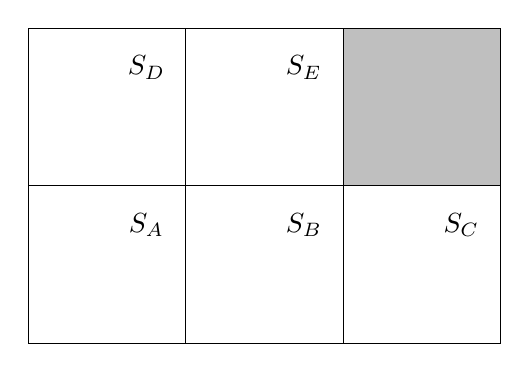
\begin{tikzpicture}
    \draw[step=2cm] (0,0) grid (6, 4);
    
    \draw[fill=white!50!gray] (4,2) rectangle (6, 4);
    
    \foreach \x/\y/\m in {
        0/1/D, 1/1/E, 
        0/0/A, 1/0/B, 2/0/C}
        \node at (2*\x + 1.5,2*\y + 1.5) {$S_\m$};

    % WRITE YOUR SOLUTION HERE
    % Be careful NOT TO DELETE THE COMMA!
    % There MUST be a comma at the end of every line
    \foreach \x/\y/\m in {
        0/0/{}, % REPLACE THE {} WITH THE VALUE FOR STATE A HERE 
        1/0/{}, % REPLACE THE {} WITH THE VALUE FOR STATE B HERE 
        2/0/{}, % REPLACE THE {} WITH THE VALUE FOR STATE C HERE 
        0/1/{}, % REPLACE THE {} WITH THE VALUE FOR STATE D HERE 
        1/1/{} % REPLACE THE {} WITH THE VALUE FOR STATE E HERE
        }  
        \node at (2*\x + 1,2*\y + 1) {$\m$};
    
    \end{tikzpicture}
    \end{center}

    
    % \begin{center}
    % \begin{tikzpicture}
    % \draw[step=2cm] (0,0) grid (8, 6);
    
    % \foreach \x/\y in {
    %     2/1, 0/2, 0/0}
    %     \draw[fill=white!50!gray] 
    %     (2*\x,2*\y) rectangle (2*\x + 2, 2*\y + 2);
    
    
    % \foreach \x/\y/\m in {
    %     0/2/I, 1/2/J, 2/2/K, 3/2/L,
    %     0/1/E, 1/1/F, 2/1/G, 3/1/H,
    %     0/0/A, 1/0/B, 2/0/C, 3/0/D}
    %     \node at (2*\x + 1.5,2*\y + 1.5) {$S_\m$};
        
    % % WRITE YOUR SOLUTION HERE
    % % Be careful NOT TO DELETE THE COMMA!
    % % There MUST be a comma at the end of every line
    % \foreach \x/\y/\m in {
    %     1/0/{}, % REPLACE THE {} WITH THE VALUE FOR STATE B HERE 
    %     2/0/{}, % REPLACE THE {} WITH THE VALUE FOR STATE C HERE 
    %     3/0/{}, % REPLACE THE {} WITH THE VALUE FOR STATE D HERE
    %     0/1/{}, % REPLACE THE {} WITH THE VALUE FOR STATE E HERE 
    %     1/1/{}, % REPLACE THE {} WITH THE VALUE FOR STATE F HERE
    %     3/1/{}, % REPLACE THE {} WITH THE VALUE FOR STATE H HERE 
    %     1/2/{}, % REPLACE THE {} WITH THE VALUE FOR STATE J HERE 
    %     2/2/{}, % REPLACE THE {} WITH THE VALUE FOR STATE K HERE 
    %     3/2/{}, % REPLACE THE {} WITH THE VALUE FOR STATE L HERE
    %     }  
    %     \node at (2*\x + 1,2*\y + 1) {$\m$};
    
    % \end{tikzpicture}
    % \end{center}
    
    
    % \part[3] What is the policy, $\pi(s)$, that corresponds to the value table you calculated above? Write one of \texttt{up}, \texttt{down}, \texttt{left}, or \texttt{right} for each state. If multiple actions are acceptable, choose the one that comes alphabetically first. For terminal states, write \texttt{terminal}. Ignore the blocked states.
    
    % \begin{center}
    % \begin{tikzpicture}
    % \draw[step=2cm] (0,0) grid (8, 6);
    
    % \foreach \x/\y in {
    %     2/1, 0/2, 0/0}
    %     \draw[fill=white!50!gray] 
    %     (2*\x,2*\y) rectangle (2*\x + 2, 2*\y + 2);
    
    
    % \foreach \x/\y/\m in {
    %     0/2/I, 1/2/J, 2/2/K, 3/2/L,
    %     0/1/E, 1/1/F, 2/1/G, 3/1/H,
    %     0/0/A, 1/0/B, 2/0/C, 3/0/D}
    %     \node at (2*\x + 1.5,2*\y + 1.5) {$S_\m$};
    
    % % WRITE YOUR SOLUTION HERE
    % % Be careful NOT TO DELETE THE COMMA!
    % % There MUST be a comma at the end of every line
    % % You only have to write up, down, left, or right.
    % % No need to write \texttt{up}
    % \foreach \x/\y/\m in {
    %     1/0/{}, % REPLACE THE {} WITH THE POLICY FOR STATE B HERE 
    %     2/0/{}, % REPLACE THE {} WITH THE POLICY FOR STATE C HERE 
    %     3/0/{}, % REPLACE THE {} WITH THE POLICY FOR STATE D HERE
    %     0/1/{}, % REPLACE THE {} WITH THE POLICY FOR STATE E HERE 
    %     1/1/{}, % REPLACE THE {} WITH THE POLICY FOR STATE F HERE
    %     3/1/{}, % REPLACE THE {} WITH THE POLICY FOR STATE H HERE
    %     1/2/{}, % REPLACE THE {} WITH THE POLICY FOR STATE J HERE 
    %     2/2/{}, % REPLACE THE {} WITH THE POLICY FOR STATE K HERE 
    %     3/2/{}, % REPLACE THE {} WITH THE POLICY FOR STATE L HERE
    %     }  
    %     \node at (2*\x + 1,2*\y + 1) {\texttt{\m}};
    
    % \end{tikzpicture}
    % \end{center}
    
    
    \clearpage
    
    \part[3] Below, we give you the value of each state one round before the convergence of \textbf{asynchronous} value iteration.\footnote{This is actually one round before the \emph{policy} convergence, not the \emph{value} convergence. The values we provide are the values after the second iteration, rounded to the nearest whole number for ease of calculation.} What is the value of each state, $V'(s)$, after another round of value iteration? Be sure to use \textbf{asynchronous} value iteration, and visit each state in \textit{reverse alphabetical order}. Ignore the blocked states. Round your \textit{answers only} to the first decimal place. \textbf{Do not round any intermediate values, including state values, when calculating your answers.}

    \begin{center}
    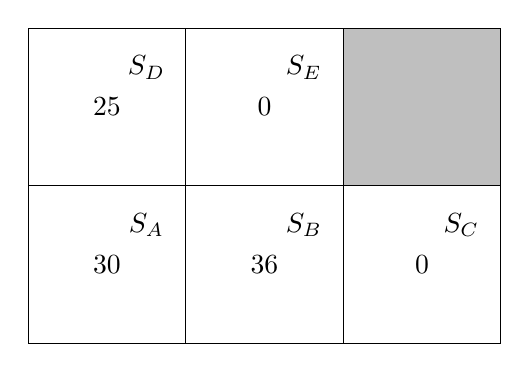
\begin{tikzpicture}
    \draw[step=2cm] (0,0) grid (6, 4);
    
    \draw[fill=white!50!gray] (4,2) rectangle (6, 4);
    
    \foreach \x/\y/\m in {
        0/1/D, 1/1/E,
        0/0/A, 1/0/B, 2/0/C}
        \node at (2*\x + 1.5,2*\y + 1.5) {$S_\m$};

    % VALUES ONE ROUND BEFORE CONVERGENCE   
    \foreach \x/\y/\m in {
        0/0/{30}, %   A  
        1/0/{36}, %   B  
        2/0/{0}, %   C  (terminal state, so no need to store value)
        0/1/{25}, %   D  
        1/1/{0}  %   E  (terminal state, so no need to store value)
        }  
        \node at (2*\x + 1,2*\y + 1) {$\m$};
    
    \end{tikzpicture}
    \end{center}
    
    % \begin{center}
    % \begin{tikzpicture}
    % \draw[step=2cm] (0,0) grid (8, 6);
    
    % \foreach \x/\y in {
    %     2/1, 0/2, 0/0}
    %     \draw[fill=white!50!gray] 
    %     (2*\x,2*\y) rectangle (2*\x + 2, 2*\y + 2);
    
    
    % \foreach \x/\y/\m in {
    %     0/2/I, 1/2/J, 2/2/K, 3/2/L,
    %     0/1/E, 1/1/F, 2/1/G, 3/1/H,
    %     0/0/A, 1/0/B, 2/0/C, 3/0/D}
    %     \node at (2*\x + 1.5,2*\y + 1.5) {$S_\m$};
    
    % % VALUES ONE ROUND BEFORE CONVERGENCE   
    % \foreach \x/\y/\m in {
    %     1/0/{22.2793}, % B
    %     2/0/{17.6604}, % C
    %     3/0/{20.60195}, % D
    %     0/1/{},  % E (terminal state, so no need to store value)
    %     1/1/{26.2819}, % F
    %     3/1/{24.248}, % H
    %     1/2/{40.4758}, % J
    %     2/2/{48.496}, % K
    %     3/2/{},  % L
    %     }  
    %     \node at (2*\x + 1,2*\y + 1) {$\m$};
    
    % \end{tikzpicture}
    % \end{center}
    
    \textbf{Your solution:}

    \begin{center}
    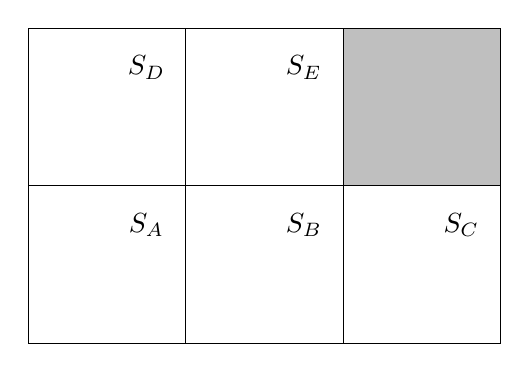
\begin{tikzpicture}
    \draw[step=2cm] (0,0) grid (6, 4);
    
    \draw[fill=white!50!gray] (4,2) rectangle (6, 4);
    
    \foreach \x/\y/\m in {
        0/1/D, 1/1/E, 
        0/0/A, 1/0/B, 2/0/C}
        \node at (2*\x + 1.5,2*\y + 1.5) {$S_\m$};

    % WRITE YOUR SOLUTION HERE
    % Be careful NOT TO DELETE THE COMMA!
    % There MUST be a comma at the end of every line
    \foreach \x/\y/\m in {
        0/0/{}, % REPLACE THE {} WITH THE VALUE FOR STATE A HERE 
        1/0/{}, % REPLACE THE {} WITH THE VALUE FOR STATE B HERE 
        2/0/{}, % REPLACE THE {} WITH THE VALUE FOR STATE C HERE 
        0/1/{}, % REPLACE THE {} WITH THE VALUE FOR STATE D HERE 
        1/1/{} % REPLACE THE {} WITH THE VALUE FOR STATE E HERE
        }  
        \node at (2*\x + 1,2*\y + 1) {$\m$};
    
    \end{tikzpicture}
    \end{center}
    
    % \begin{center}
    % \begin{tikzpicture}
    % \draw[step=2cm] (0,0) grid (8, 6);
    
    % \foreach \x/\y in {
    %     2/1, 0/2, 0/0}
    %     \draw[fill=white!50!gray] 
    %     (2*\x,2*\y) rectangle (2*\x + 2, 2*\y + 2);
    
    
    % \foreach \x/\y/\m in {
    %     0/2/I, 1/2/J, 2/2/K, 3/2/L,
    %     0/1/E, 1/1/F, 2/1/G, 3/1/H,
    %     0/0/A, 1/0/B, 2/0/C, 3/0/D}
    %     \node at (2*\x + 1.5,2*\y + 1.5) {$S_\m$};
        
    % % WRITE YOUR SOLUTION HERE
    % % Be careful NOT TO DELETE THE COMMA!
    % % There MUST be a comma at the end of every line
    % \foreach \x/\y/\m in {
    %     1/0/{}, % REPLACE THE {} WITH THE VALUE FOR STATE B HERE 
    %     2/0/{}, % REPLACE THE {} WITH THE VALUE FOR STATE C HERE 
    %     3/0/{}, % REPLACE THE {} WITH THE VALUE FOR STATE D HERE
    %     0/1/{}, % REPLACE THE {} WITH THE VALUE FOR STATE E HERE 
    %     1/1/{}, % REPLACE THE {} WITH THE VALUE FOR STATE F HERE
    %     3/1/{}, % REPLACE THE {} WITH THE VALUE FOR STATE H HERE
    %     1/2/{}, % REPLACE THE {} WITH THE VALUE FOR STATE J HERE 
    %     2/2/{}, % REPLACE THE {} WITH THE VALUE FOR STATE K HERE 
    %     3/2/{}, % REPLACE THE {} WITH THE VALUE FOR STATE L HERE
    %     } 
    %     \node at (2*\x + 1,2*\y + 1) {\texttt{\m}};
    
    % \end{tikzpicture}
    % \end{center}
    
    
    % \clearpage
    \vspace{1em}
    
    \part[3] What is the policy, $\pi^*(s)$, that corresponds to $V'(s)$? Write one of \texttt{up}, \texttt{down}, \texttt{left}, or \texttt{right} for each state. If multiple actions are acceptable, choose the one that comes alphabetically first. For terminal states, write \texttt{terminal}. Ignore the blocked states.

    \begin{center}
    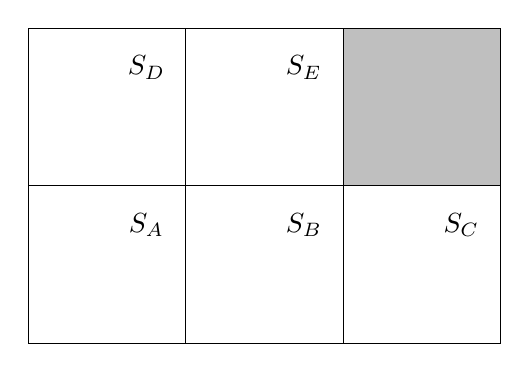
\begin{tikzpicture}
    \draw[step=2cm] (0,0) grid (6, 4);
    
    \draw[fill=white!50!gray] (4,2) rectangle (6, 4);
    
    \foreach \x/\y/\m in {
        0/1/D, 1/1/E,
        0/0/A, 1/0/B, 2/0/C}
        \node at (2*\x + 1.5,2*\y + 1.5) {$S_\m$};

    % WRITE YOUR SOLUTION HERE
    % Be careful NOT TO DELETE THE COMMA!
    % There MUST be a comma at the end of every line
    \foreach \x/\y/\m in {
        0/0/{}, % REPLACE THE {} WITH THE VALUE FOR STATE A HERE 
        1/0/{}, % REPLACE THE {} WITH THE VALUE FOR STATE B HERE 
        2/0/{}, % REPLACE THE {} WITH THE VALUE FOR STATE C HERE 
        0/1/{}, % REPLACE THE {} WITH THE VALUE FOR STATE D HERE 
        1/1/{} % REPLACE THE {} WITH THE VALUE FOR STATE E HERE
        }  
        \node at (2*\x + 1,2*\y + 1) {$\m$};
    
    \end{tikzpicture}
    \end{center}
    
    % \begin{center}
    % \begin{tikzpicture}
    % \draw[step=2cm] (0,0) grid (8, 6);
    
    % \foreach \x/\y in {
    %     2/1, 0/2, 0/0}
    %     \draw[fill=white!50!gray] 
    %     (2*\x,2*\y) rectangle (2*\x + 2, 2*\y + 2);
    
    
    % \foreach \x/\y/\m in {
    %     0/2/I, 1/2/J, 2/2/K, 3/2/L,
    %     0/1/E, 1/1/F, 2/1/G, 3/1/H,
    %     0/0/A, 1/0/B, 2/0/C, 3/0/D}
    %     \node at (2*\x + 1.5,2*\y + 1.5) {$S_\m$};
    
    % % WRITE YOUR SOLUTION HERE
    % % Be careful NOT TO DELETE THE COMMA!
    % % There MUST be a comma at the end of every line
    % % You only have to write up, down, left, or right.
    % % No need to write \texttt{up}
    % \foreach \x/\y/\m in {
    %     1/0/{}, % REPLACE THE {} WITH THE POLICY FOR STATE B HERE 
    %     2/0/{}, % REPLACE THE {} WITH THE POLICY FOR STATE C HERE 
    %     3/0/{}, % REPLACE THE {} WITH THE POLICY FOR STATE D HERE
    %     0/1/{}, % REPLACE THE {} WITH THE POLICY FOR STATE E HERE 
    %     1/1/{}, % REPLACE THE {} WITH THE POLICY FOR STATE F HERE
    %     3/1/{}, % REPLACE THE {} WITH THE POLICY FOR STATE H HERE
    %     1/2/{}, % REPLACE THE {} WITH THE POLICY FOR STATE J HERE 
    %     2/2/{}, % REPLACE THE {} WITH THE POLICY FOR STATE K HERE 
    %     3/2/{}, % REPLACE THE {} WITH THE POLICY FOR STATE L HERE
    %     } 
    %     \node at (2*\x + 1,2*\y + 1) {\texttt{\m}};
    
    % \end{tikzpicture}
    % \end{center}
    

\end{parts}

\clearpage    \newpage
\sectionquestion{Q-Learning}

Let's consider an environment that is similar to the grid world we saw before, but has more states:

\begin{center}
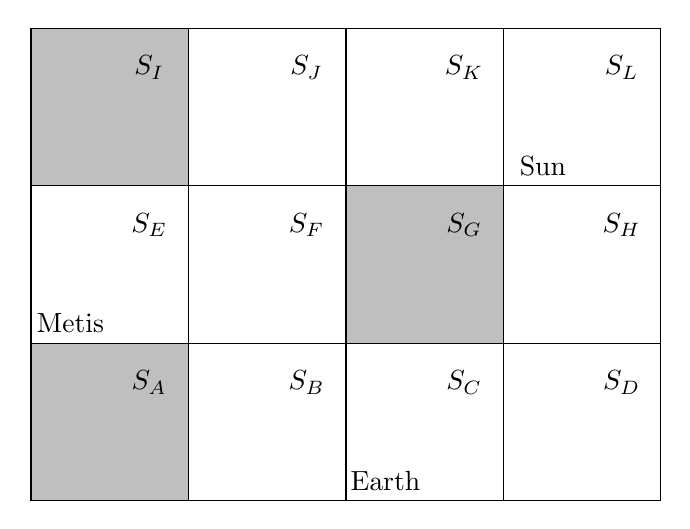
\begin{tikzpicture}
\draw[step=2cm] (0,0) grid (8, 6);

\node at (4.5, 0.25) {Earth};
\node at (6.5, 4.25) {Sun};
\node at (0.5, 2.25) {Metis};

\foreach \x/\y in {
    2/1, 0/2, 0/0}
    \draw[fill=white!50!gray] 
    (2*\x,2*\y) rectangle (2*\x + 2, 2*\y + 2);


\foreach \x/\y/\m in {
    0/2/I, 1/2/J, 2/2/K, 3/2/L,
    0/1/E, 1/1/F, 2/1/G, 3/1/H,
    0/0/A, 1/0/B, 2/0/C, 3/0/D}
    \node at (2*\x + 1.5,2*\y + 1.5) {$S_\m$};

\end{tikzpicture}
\end{center}

This time, however, suppose we \textbf{don't know} the reward function or the transition probability between states. Some rules for this setup are:

\begin{enumerate}
    \item Each grid cell is a state $S_A, S_B, \hdots , S_L$ corresponding to a position in the solar system.
    \item The action space of the agent is: $\{\texttt{up}, \texttt{down}, \texttt{left}, \texttt{right}\}$.
    \item If the agent hits the edge of the board, it remains in the same state. It is not possible to move into blocked states, which are shaded grey, since they contain other planets.
    \item The start state is $S_C$ (Earth). The terminal states include both the $S_L$ (Sun) and $S_E$ (asteroid Metis).
    \item Use the discount factor $\gamma = 0.9$ and learning rate $\alpha=0.1$.
\end{enumerate}

We will go through three iterations of Q-learning in this section. Initialize $Q(s,a)$ as below:

\begin{table}[h!]
\centering
 \begin{tabular}{||c c c c c c c c c c c c c||} 
 \hline
 $a \setminus s$ & $S_A$ & $S_B$ & $S_C$ & $S_D$ & $S_E$ & $S_F$ & $S_G$ & $S_H$ & $S_I$ & $S_J$ & $S_K$ & $S_L$ \\ [0.4ex] 
 \hline\hline
 Up    & 0.4 & 0.1 & 0.1 & 0.7 & 0.0 & 0.9 & 0.7 & 0.8 & 0.0 & 0.1 & 0.8 & 0.8 \\ 
 Down  & 1.0 & 0.8 & 0.2 & 0.5 & 0.1 & 0.2 & 0.7 & 0.2 & 1.0 & 0.9 & 0.1 & 0.3 \\ 
 Left  & 0.9 & 0.4 & 0.3 & 0.4 & 0.9 & 0.6 & 0.5 & 0.1 & 0.2 & 0.3 & 0.9 & 0.1 \\
 Right & 0.3 & 0.8 & 0.3 & 0.2 & 0.0 & 0.2 & 0.2 & 0.3 & 0.9 & 0.4 & 0.2 & 0.3 \\  [1ex] 
 \hline
 \end{tabular}
\end{table}

\begin{parts}
\part[1] \sall If the agent were to act greedily, what action(s) could it take at this time from state $S_C$?

{
\checkboxchar{$\Box$} \checkedchar{$\blacksquare$}
\begin{checkboxes}
    \choice \texttt{up}
    \choice \texttt{down}
    \choice \texttt{left}
    \choice \texttt{right}
\end{checkboxes}
}


\clearpage

\part[1] Beginning at state $S_C$, you take the action \texttt{right} and receive a reward of 0. You are now in state $S_D$. What is the new value for $Q(S_C, \texttt{right})$, assuming the update for deterministic transitions? If needed, round your answer to the fourth decimal place.

\begin{your_solution}[title={$Q(S_C, \texttt{right})$},height=2cm,width=4cm]
\end{your_solution}

\part[1] What is the new value for $Q(S_C, \texttt{right})$, using the temporal difference error update? If needed, round your answer to the fourth decimal place.

\begin{your_solution}[title={$Q(S_C, \texttt{right})$},height=2cm,width=4cm]
\end{your_solution}

\part[1] \sall Assume your run has brought you to state $S_H$ with no updates to the Q-function in the process. If the agent were to act greedily, what action(s) could it take at this time?

{
\checkboxchar{$\Box$} \checkedchar{$\blacksquare$}
\begin{checkboxes}
    \choice \texttt{up}
    \choice \texttt{down}
    \choice \texttt{left}
    \choice \texttt{right}
\end{checkboxes}
}


\part[1] Beginning at state $S_H$, you take the action \texttt{up}, receive a reward of +25, and the run terminates. What is the new value for $Q(S_H, \texttt{up})$, assuming the update for deterministic transitions? If needed, round your answer to the fourth decimal place.

\begin{your_solution}[title={$Q(S_H, \texttt{up})$},height=2cm,width=4cm]
\end{your_solution}

\part[1] What is the new value for $Q(S_H, \texttt{up})$, using the temporal difference error update? If needed, round your answer to the fourth decimal place.

\begin{your_solution}[title={$Q(S_H, \texttt{up})$},height=2cm,width=4cm]
\end{your_solution}

\clearpage

\part[1] \sall You start from state $S_C$ again since the previous run terminated. Assume you manage to make it to state $S_F$ with no updates to the Q-function. If the agent were to act greedily, what action(s) could it take at this time?

{
\checkboxchar{$\Box$} \checkedchar{$\blacksquare$}
\begin{checkboxes}
    \choice \texttt{up}
    \choice \texttt{down}
    \choice \texttt{left}
    \choice \texttt{right}
\end{checkboxes}
}


\part[1] Beginning at state $S_F$, you take the action \texttt{left}, receive a reward of -50, and the run terminates. What is the new value for $Q(S_F, \texttt{left})$, assuming the update for deterministic transitions? If needed, round your answer to the fourth decimal place.

\begin{your_solution}[title={$Q(S_F, \texttt{left})$},height=2cm,width=4cm]
\end{your_solution}

\part[1] What is the new value for $Q(S_F, \texttt{left})$, using the temporal difference error update? If needed, round your answer to the fourth decimal place.

\begin{your_solution}[title={$Q(S_F, \texttt{left})$},height=2cm,width=4cm]
\end{your_solution}

\end{parts}

\clearpage    \newpage
\sectionquestion{Empirical Questions}

The following parts should be completed after you work through the programming portion of this assignment. 

\begin{parts}
    \part[4] Run the actor critic algorithm. Show the two plots you produced: the training and evaluation rewards over episodes. 
    
    \begin{your_solution}[title=Plot of Training Rewards over episodes, height=10cm]
        % YOUR ANSWER 
    
    \end{your_solution}
    
    \begin{your_solution}[title=Plot of Testing Rewards over episodes, height=10cm]
        % YOUR ANSWER
   
    \end{your_solution}
    
    % \begin{your_solution}[title=Comment,height=5cm]
    %     % YOUR ANSWER 
    % \end{your_solution}

    \part[4] Evaluate your agent after training to get videos of it playing Pong. Comment on your findings from the video. For example, what behaviors did it learn? what mistakes does it still make? how do you think these mistakes could be addressed?
    
    \begin{your_solution}[title=Findings from video of the game, height=10cm]
        % YOUR ANSWER 
    
    \end{your_solution}
    
    
    \clearpage
\end{parts}

    \clearpage    \newpage
\newpage
\section{Collaboration Questions}
After you have completed all other components of this assignment, report your answers to these questions regarding the collaboration policy. Details of the policy can be found \href{http://www.cs.cmu.edu/~mgormley/courses/10601/index.html#syllabus}{here}.
\begin{enumerate}
    \item Did you receive any help whatsoever from anyone in solving this assignment? If so, include full details.
    \item Did you give any help whatsoever to anyone in solving this assignment? If so, include full details.
    \item Did you find or come across code that implements any part of this assignment? If so, include full details.
\end{enumerate}

\begin{your_solution}[height=6cm]
% YOUR ANSWER 

\end{your_solution}
    \newpage
    \end{questions}
    
\section{Programming [68 Points]}
\label{sec:code}

Your goal in this assignment is to implement the Advantage Actor Critic (A2C) algorithm to train an agent to play the Atari Pong game. You will implement all the functions needed to optimize the policy and value networks and to deploy your agent in the Pong environment. We provide a simplified version of the Pong environment for you to use. The program you write will be automatically graded using Gradescope.

\subsection{Libraries and Setup (IMPORTANT)}
In this assignment, we \textbf{highly} recommend you use a conda environment, as we will be using several libraries (e.g. \lstinline{gymnasium}, \lstinline{ale_py}, \lstinline{pytorch}). You can set up a conda environment called ``HW8" as such:

\begin{lstlisting}[language=Shell]
$ conda create -n HW8 python=3.12
$ conda activate HW8
\end{lstlisting}

To deactivate the conda environment, use the command:
\begin{lstlisting}[language=Shell]
$ conda deactivate
\end{lstlisting}
Once you have created this environment, you can activate/deactivate this environment as much as you want without having to recreate it each time (assuming you did not also delete the environment).

We have provided a \lstinline{requirements.txt} file to make library installation straightforward. To install the libraries, use the command:

\begin{lstlisting}[language=Shell]
$ pip install -r requirements.txt
\end{lstlisting}

\subsection{The Pong Environment}
In this assignment, you will be using the Arcade Learning Environment (ALE), a library with a set of Atari games that run on top of Gymnasium, a library for reinforcement learning. Specifically, your goal is to train an agent to play \href{https://en.wikipedia.org/wiki/Pong}{Pong}, one of the most popular Atari games. You are provided with code that wraps the ALE/Gymnasium Pong environment to simplify its API and to help you focus on the algorithm implementation.

In Pong, there are two paddles that bounce a ball back and forth from left to right. You play as the paddle on the right, and your objective is to continuously return the ball. The paddle that misses the ball first loses and receives a reward of -1, while the other wins and receives a reward of 1, and the episode terminates. There are no other rewards. 

The state of the environment is represented by a vector of size 6 which contains:
\begin{itemize}
    \item The position of your paddle along the $y$ axis
    \item The position of the opponent's paddle along the $y$ axis
    \item The position of the ball along the $x$ axis
    \item The position of the ball along the $y$ axis
    \item The velocity of the ball along the $x$ axis
    \item The velocity of the ball along the $y$ axis
\end{itemize}
    The actions the agent can take at any state are defined as $\{0, 1\}$, corresponding to the actions: (0) move down, and (1) move up.

\begin{figure}
\centering
\includegraphics[scale=1]{figs/Pong_frame.png}
\caption{Rendered frame of the Pong environment. You play as the green paddle (to the right), and your opponent is the orange paddle (to the left). The white pixel in the bottom left is the ball.}
\end{figure}

\subsection{The Advantage Actor Critic Algorithm (A2C)}

\subsubsection{Background: The Reinforcement Learning Paradigm}

In reinforcement learning (RL), we face a fundamental challenge that distinguishes it from supervised learning: \textit{we do not have labeled data}. Instead of receiving input-output pairs $(x, y)$, an RL agent must learn from sequential interactions with an environment, receiving only sparse reward signals that may be delayed in time (maybe an action taken at timestep $t$ leads to high rewards at timestep $t+1000$). With this information, the agent must discover which actions lead to desirable outcomes through trial and error.

\subsubsection{The RL Objective: Expected Reward Maximization}

The goal in RL is to find a policy $\pi_\theta(a|s)$ that maximizes the expected cumulative discounted reward:
\begin{equation}
J(\theta) = \mathbb{E}_{\tau \sim \pi_\theta} \left[ \sum_{t=0}^{T} \gamma^t r_t \right] = \mathbb{E}_{\tau \sim \pi_\theta} [R(\tau)]
\end{equation}
where $\tau = (s_0, a_0, r_0, s_1, a_1, r_1, \ldots)$ is a trajectory or episode, $\gamma \in [0,1]$ is the discount factor, and the expectation is taken over trajectories or episodes obtained by deploying the policy $\pi_\theta$ on the environment.

\subsubsection{The REINFORCE Algorithm}

To optimize $J(\theta)$ using gradient ascent, we need to compute $\nabla_\theta J(\theta)$. Using the likelihood ratio trick, we can derive:

\begin{align}
\nabla_\theta J(\theta)
&= \nabla_\theta \mathbb{E}_{\tau \sim \pi_\theta} [R(\tau)] \\
&= \nabla_\theta \sum_{\tau} [R(\tau) p_\theta(\tau)] \\
&= \sum_{\tau} [R(\tau) \nabla_\theta p_\theta(\tau)] \\
&= \sum_{\tau} [R(\tau) p_\theta(\tau) \frac{\nabla_\theta p_\theta(\tau)}{p_\theta(\tau)}] \\
&= \sum_{\tau} [R(\tau) p_\theta(\tau) \nabla_\theta \log{p_\theta(\tau)})] \\
&= \mathbb{E}_{\tau \sim \pi_\theta} [R(\tau) \nabla_\theta \log p_\theta(\tau)] \\
&= \mathbb{E}_{\tau \sim \pi_\theta} \left[ R(\tau) \sum_{t=0}^{T} \nabla_\theta \log \pi_\theta(a_t | s_t) \right] \\
&= \mathbb{E}_{\tau \sim \pi_\theta} \left[ \sum_{t=0}^{T} \nabla_\theta \log \pi_\theta(a_t | s_t) \sum_{t'=t}^{T} \gamma^{t'} r_{t'} \right]
\end{align}

The last step uses the fact that actions at time $t$ cannot influence rewards received before time $t$. Defining the return from time $t$ as $G_t = \sum_{t'=t}^{T} \gamma^{t'-t} r_{t'}$, we obtain the \textbf{REINFORCE policy gradient}:
\begin{equation}
\nabla_\theta J(\theta) = \mathbb{E}_{\tau \sim \pi_\theta} \left[ \sum_{t=0}^{T} \nabla_\theta \log \pi_\theta(a_t | s_t) \cdot G_t \right]
\end{equation}

In practice, we estimate this expectation by sampling trajectories (also known as Monte Carlo estimation).

\subsubsection{From REINFORCE to A2C}

While REINFORCE is theoretically sound, it suffers from high variance. The returns $G_t$ and score vectors $\nabla_\theta\log\pi_\theta$ can vary dramatically between trajectories, leading to noisy gradient estimates and slow, unstable learning.

\textbf{Advantage Actor-Critic (A2C)} addresses this issue through baseline subtraction. Instead of using raw returns $G_t$, A2C uses the \textbf{advantage function}:
\begin{equation}
A(s_t, a_t) = Q(s_t, a_t) - V(s_t)
\end{equation}
where $V(s_t)$ is the value function (expected return from state $s_t$) and $Q(s_t, a_t)$ is the Q-value function (expected return from taking action $a_t$ at state $s_t$). The advantage measures how much better action $a_t$ is compared to the average action in state $s_t$. Replacing raw returns with advantages reduces variance without introducing bias because $\mathbb{E}[V(s_t)]$ is constant with respect to $a_t$.

The gradient becomes:
\begin{equation}
\nabla_\theta J(\theta) = \mathbb{E} \left[ \sum_{t=0}^{T} \nabla_\theta \log \pi_\theta(a_t | s_t) \cdot A(s_t, a_t) \right]
\end{equation}

To estimate advantages, A2C learns a separate \textbf{critic} network $V_\phi(s)$ to approximate the value function. We can then estimate the advantage using:
\begin{equation}
A(s_t, a_t) \approx r_t + \gamma V_\phi(s_{t+1}) - V_\phi(s_t)
\end{equation}
Remember that $Q(s_t, a_t) = r_t + \gamma V(s_{t+1})$ where $r_t$ is the reward obtained after taking action $a_t$ at state $s_t$. This allows us to obtain a gradient estimate for every step rather than once per full trajectory, improving sample efficiency.


\subsubsection{N-Step Returns: Balance between bias and variance}

While 1-step TD learning (using $r_t + \gamma V_\phi(s_{t+1})$) provides low-variance estimates, it can be biased when the value function is inaccurate. Conversely, Monte Carlo returns (full trajectories) are unbiased but high-variance. \textbf{N-step returns} provide a middle ground that can improve learning.

The \textbf{N-step return} from time $t$ is defined as:
\begin{equation} \label{eq:n-step-returns}
G_t^{(n)} = \sum_{k=0}^{n-1} \gamma^k r_{t+k} + \gamma^n V_\phi(s_{t+n})
\end{equation}

This sums the actual rewards for $n$ steps, then bootstraps from the value estimate at step $t+n$. The N-step advantage estimate becomes:
\begin{equation}
A_t^{(n)} = G_t^{(n)} - V_\phi(s_t) = \sum_{k=0}^{n-1} \gamma^k r_{t+k} + \gamma^n V_\phi(s_{t+n}) - V_\phi(s_t)
\end{equation}

\textbf{Benefits of N-step returns:}
\begin{itemize}
\item \textbf{Bias-variance tradeoff}: Larger $n$ reduces bias (relying less on potentially inaccurate value estimates) but increases variance.
\item \textbf{Faster credit assignment}: Rewards propagate $n$ steps backward in a single update rather than just 1 step, accelerating learning in sparse-reward environments.
\item \textbf{Better gradient quality}: Advantages based on actual observed rewards tend to provide more reliable policy gradient signals.
\end{itemize}

Similarly, the critic's target becomes the N-step return $G_t^{(n)}$ instead of the 1-step TD target.

\subsubsection{A2C Algorithm Summary}

The \textbf{A2C algorithm} maintains two networks that are trained jointly:

\begin{itemize}
\item \textbf{Actor} $\pi_\theta(a|s)$: The policy network, parameterized by $\theta$. Updated using policy gradients with N-step advantage estimates:
\begin{equation} \label{eq:policy_loss}
\theta \leftarrow \theta + \eta_\textit{policy} \nabla_\theta \log \pi_\theta(a_t | s_t) \cdot A_t^{(n)}
\end{equation}

\item \textbf{Critic} $V_\phi(s)$: The value network, parameterized by $\phi$. Updated to minimize the squared error between predictions and N-step returns:
\begin{equation} \label{eq:value_loss}
\phi \leftarrow \phi - \eta_\textit{value} \nabla_\phi \left(V_\phi(s_t) - G_t^{(n)}\right)^2
\end{equation}
\end{itemize}

Both networks need to be updated synchronously after collecting experience for $B$ episodes.

\subsection{File Structure}

The handout contains the following files:

\begin{itemize}
    \item \texttt{environment.py}: Pong Environment (provided for you)
    \item \texttt{agent.py}: File in which you will implement the A2C algorithm
    \item \texttt{utils.py}: Utility functions for plotting rewards and setting random seeds (provided for you)
    \item \texttt{test\_runner.py}: Script to run unit tests to debug your implementation
    \item \texttt{test\_cases}: Unit tests
    \item \texttt{test\_data}: Auxiliary data for the unit tests
    \item \texttt{requirements.txt}: Dependencies for the assignment
\end{itemize}


\subsection{TODOs}

You will need to implement the following in \texttt{agent.py}

\begin{itemize}
    \item \texttt{Policy}: Pytorch module that models the policy as a neural network
    \item \texttt{Value}: Pytorch module that models the value function as a neural network
    \item \texttt{Agent.get\_action}: Method that samples an action from the policy 
    \item \texttt{Agent.n\_step\_returns}: Method that calculates the N-Step Returns given a sequence of rewards and value estimates
    \item \texttt{Agent.policy\_loss}: Method that calculates the loss we will minimize to optimize the parameters of the policy network
    \item \texttt{Agent.value\_loss}: Method that calculates the loss we will minimize to optimize the parameters of the value network
    \item \texttt{Agent.update\_policy}: Method that takes a step of gradient descent to update the parameters of the policy network
    \item \texttt{Agent.update\_value}: Method that takes a step of gradient descent to update the parameters of the value network
    \item \texttt{deploy\_agent}: Function that deploys the agent in the Pong environment
\end{itemize}

There are other initializations you need to implement which are marked with TODOs in \texttt{agent.py}. You need to complete those TODOs to train and evaluate your agent; see the starter code for details.

\subsection{The Pong Environment API}
The Pong environment provides the following API to interact with it.
\begin{itemize}
    \item \texttt{\_\_init\_\_(max\_steps, record)}: Initializes the environment such that each episode takes at most \texttt{max\_steps} number of steps. Setting \texttt{record = True} allows you to record and save a video of a game. Only set \texttt{record = True} when evaluating the agent, otherwise training will be too slow.
    
    \item \texttt{reset()}: Resets the environment and returns the initial state.
    
    \item \texttt{step(action)}: Take a step in the environment with the given action. \texttt{action} must be $0$ (down) or $1$ (up). \texttt{step(action)} returns a tuple of $(\texttt{state}, \texttt{reward}, \texttt{terminated}, \texttt{truncated})$ which are the next state, the reward observed, a boolean indicating whether the episode has terminated, and a boolean indicating if we reached the maximum number of steps. The \texttt{state} will be the new state that the agent is in after taking its specified action. If you observe \texttt{terminated = True} or \texttt{truncated = True} then you should \texttt{reset} the environment and end the episode. Failure to do so will result in undefined behavior.
\end{itemize}

\subsection{Implementation Details}

\paragraph{Policy and Value Networks}
You will implement two networks, a policy network and a value network, each with exactly two hidden linear layers of size 256 (any other architectures will not pass the autograder tests). Use ReLU activations in between layers.

The policy network should return the action logits. Do not apply a softmax activation on the outputs of the network (this will cause numerical instability later when we calculate the log probabilities for the policy loss implementation).

\paragraph{Getting actions from the policy}
Use \texttt{torch.nn.functional.softmax} and \texttt{torch.multinomial} to sample from the logits returned by the policy network.

\paragraph{N-Step Returns efficient implementation}
Review the HW8 recitation for instructions/hints on how to calculate the N-Step Returns. This function should implement equation \ref{eq:n-step-returns}. Pay special attention to how you are supposed to handle values for terminal states. If $s_t$ is a terminal state, you should use $V(s_t) = 0$ (hint: remember that the \texttt{step()} method in the environment returns whether the new state is a terminal state)

\paragraph{Policy Loss}
This function should return $-\log \pi_\theta(a_t | s_t) \cdot A_t^{(n)}$, so that when we perform backpropagation on this loss we get the gradient that shows up at end of equation \ref{eq:policy_loss}. Remember that gradient descent is used to minimize an objective function. Therefore if we want to maximize the advantage weighted log probabilities, we can minimize the negative advantage weighted log probabilities.

To calculate the advantages, you will need to calculate the N-Step Returns and the value for the current state. Call your value network to get value estimates for the current and next states. Review the HW8 recitation for instructions/hints on how to stop the gradient propagation through the value network. Here we are using the value network only to get the advantages. We do not want to back-propagate the loss through the value network on this function. Use a value of $N=10$ for the N-Step Returns.

Once you have the advantages you are going to need the log probabilities of the actions taken. Review the HW8 recitation for instructions/hints on how to calculate these in a numerically stable way.

\paragraph{Value Loss}
This function should return $\left(V_\phi(s_t) - G_t^{(n)}\right)^2$, so that when we perform backpropagation on this loss we get the gradient that shows up at end of equation \ref{eq:value_loss}: .

To calculate the loss, you will need the N-Step Returns and the value for the current state. Call your value network to get value estimates for the current and next states. Review the HW8 recitation for instructions/hints on how to stop the gradient propagation. Here we only want to back-propagate through the value estimates for the current state. Use a value of $N=10$ for the N-Step Returns. You can use \texttt{torch.nn.functional.mse\_loss} to get the average MSE for all timesteps.

\paragraph{Update Policy and Value}
This methods are really simple to implement. You just need to use the optimizers to take a gradient descent step and then make sure to set all gradients to zero. Only set gradient to zero inside this function, which gets called after several back propagation calls. In this assignment we are accumulating gradients over several trajectories to make learning more stable. We only want to set gradients to zero \textit{after} taking a step with the optimizer.

\paragraph{Deploying the Agent}
Review \texttt{environment.py} for guidance on how to interact with the environment. The handout has comments that will guide you through the implementation of this function. Pay close attention to the data types and shapes of the objects this function should return. Ignoring this will cause problems in other parts of your code.

\subsection{Running the Agent}

\begin{tabbing}
\=\texttt{\$ \textbf{python} agent.\textbf{py} [args\dots]}
\end{tabbing}

where above \texttt{[args\dots]} is a placeholder for command-line arguments: \texttt{<max-steps>} \texttt{<gamma>} \texttt{<train-episodes>} \texttt{<lr>} \texttt{<batch-size>} \texttt{<store-every>} \texttt{<eval-only>} \texttt{<eval-every>} \texttt{<eval-episodes>}. These arguments are described in detail below:
\begin{enumerate}
    \item \texttt{<max-steps >}: Maximum steps per episode (default: 300)
    \item \texttt{<gamma>}: Discount factor (default: 0.98).
    \item \texttt{<train-episodes>}: Total number of training episodes (default: 30000).
    \item \texttt{<lr>}: Learning rate (default: 0.0003)
    \item \texttt{<batch-size>}: Episodes for each policy and value network update (default: 4).
    \item \texttt{<store-every>}: Episodes between each checkpoint (default: 2000).
    \item \texttt{<eval-only>}:  Flag to record a video of agent playing (default: False). If set to True, the agent will not be trained. Use only after training an agent.
    \item \texttt{<eval-every>}: Training episodes between evaluation episodes (default: 500).
    \item \texttt{<eval-episodes>}: Number of episodes per evaluation (default: 20).
\end{enumerate}

Run the following command to train your agent (use the default hyperparameters). This should take approximately 30 minutes to run on a CPU.

\begin{lstlisting}[language=Shell]
    $python agent.py 
\end{lstlisting}

Your program should produce two plots, one with the training rewards for every episode, and another one with the mean evaluation rewards across \texttt{eval-episodes} sampled every \texttt{eval-every} training episodes. 

After training your agent, run the following command to record a set of videos of the agent playing Pong!

\begin{lstlisting}[language=Shell]
    $python agent.py --eval-only
\end{lstlisting}

You program will print which video had the longest game in which your agent won. Feel free to skim over the other videos as well to answer the empirical questions.

\subsection{Testing}

The autograder will use the following commands to test your implementation:

\begin{lstlisting}[language=Shell]
$python agent.py 300 0.98 30000 0.0003 4 2000 False 500 20
 \ 4 200 0.05 0.99 0.01 1 500 
\end{lstlisting}

% \subsection{Debugging Tips}\label{subsec:debugging}

% To help with debugging, we have provided the option for printing each step of the Q-learning train function based on the reference output for the Grid World environment. We created this output by adding the \texttt{debug=True} argument when initializing the Grid World environment. You may do the same to compare your output against ours.

% We recommend first checking your outputs based on a run with extremely simple parameters and without experience replay. Remember to set \texttt{<epsilon>=0} so the program is run without the epsilon-greedy strategy.

% We have provided output on the Grid World for the following simple command:

% \begin{lstlisting}[language=Shell]
% $ python q_learning.py gw tile gw_params1_weight.txt \
%   gw_params1_returns.txt 1 1 0.0 1 1 0 0 0
% \end{lstlisting}

% Once this works, you can change the parameters to be slightly more complex (such as the ones we have below), and check with our calculations again:

% \begin{lstlisting}[language=Shell]
% $ python q_learning.py gw tile gw_params2_weight.txt gw_params2_returns.txt \
%   3 5 0.0 0.9 0.01 0 0 0
% \end{lstlisting}

% The logs for both of the above commands should be in \texttt{reference\_output/gw\_simple.log} and \texttt{reference\_output/gw.log}, respectively.

% In addition, we have provided \texttt{mc\_weight.txt} and \texttt{mc\_returns.txt} in the handout, which are generated using the following parameters:
% \begin{itemize}
%     \item \texttt{<env>}: \texttt{mc}
%     \item \texttt{<mode>}: \texttt{tile}
%     \item \texttt{<episodes>}: \texttt{25}
%     \item \texttt{<max\_iterations>}: \texttt{200}
%     \item \texttt{<epsilon>}: \texttt{0.0}
%     \item \texttt{<gamma>}: \texttt{0.99}
%     \item \texttt{<learning\_rate>}: \texttt{0.005}
%     \item \texttt{<replay\_enabled>}: \texttt{0}
%     \item \texttt{<buffer\_size>}: \texttt{0}
%     \item \texttt{<batch\_size>}: \texttt{0}
% \end{itemize}

% Example command:
% \begin{lstlisting}[language=Shell]
% $ python q_learning.py mc tile mc_params2_weight.txt \
%  mc_params2_returns.txt 25 200 0.0 0.99 0.005 0 0 0
% \end{lstlisting}

% For your convenience, we have provided a file \texttt{check.py} in the handout that will generate and compare your reward and weight outputs to all the reference outputs provided in the \texttt{reference\_output} folder. See the comment at the top of the file for instructions on running these checks.

% For all checks:
% \begin{lstlisting}[language=Shell]
% $ python -m unittest check
% \end{lstlisting}

% For a specific example (in this case Mountain Car with tile features, the command given earlier on this page):
% \begin{lstlisting}[language=Shell]
% $ python -m unittest check.MCTile
% \end{lstlisting}

\subsection{Gradescope Submission}

You should submit your \texttt{agent.py} to Gradescope.
\textbf{Any other files uploaded will be discarded or reverted back to the original version provided in the handout.}
Do \textit{not} use other file names.\end{document}